\section{WSe2}

	\subsection{Introduction}
	
		$WSe2$ is a TMDC material very similar to the $WS_2$. The main difference is its bandgap which for monolayer is about 1.65 eV. Its crystal structure is the same as the other TDMCs as outlined in \ref{sec:Introduction}. The electronic structure can be seen in Figure \ref{fig:WSe2BandStructureWSe2WS2}
		
\begin{figure}
	\begin{center}
		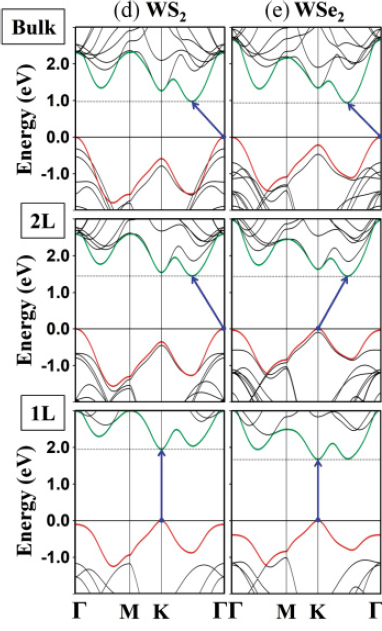
\includegraphics[scale=0.5]{WSe2/WSe2BandStructureWSe2WS2.png}
		\caption{$WS_2$ and $WSe_2$ electronic band structure for 1, 2 and many layers (bulk)}
		\label{fig:WSe2BandStructureWSe2WS2}
	\end{center}
\end{figure}
	
	\subsection{Results}
	
	A typical PL and Raman spectrum can be seen in Figure \ref{fig:WSe2PLRamanSpectra}. The PL peak is mostly symmetrical with little to no trion component as seen in $WS_2$ flakes. The peak is centred at around 1.645 eV with FWHM of 66 meV. The Raman peak around 250 $cm^{-1}$ is a convolution of 2 peaks, a $E^1_{2g}$ and $A_{1g}$ peaks.  
	
\begin{figure}[!h]
	\begin{center}
		\begin{subfigure}[b]{0.4\textwidth}
			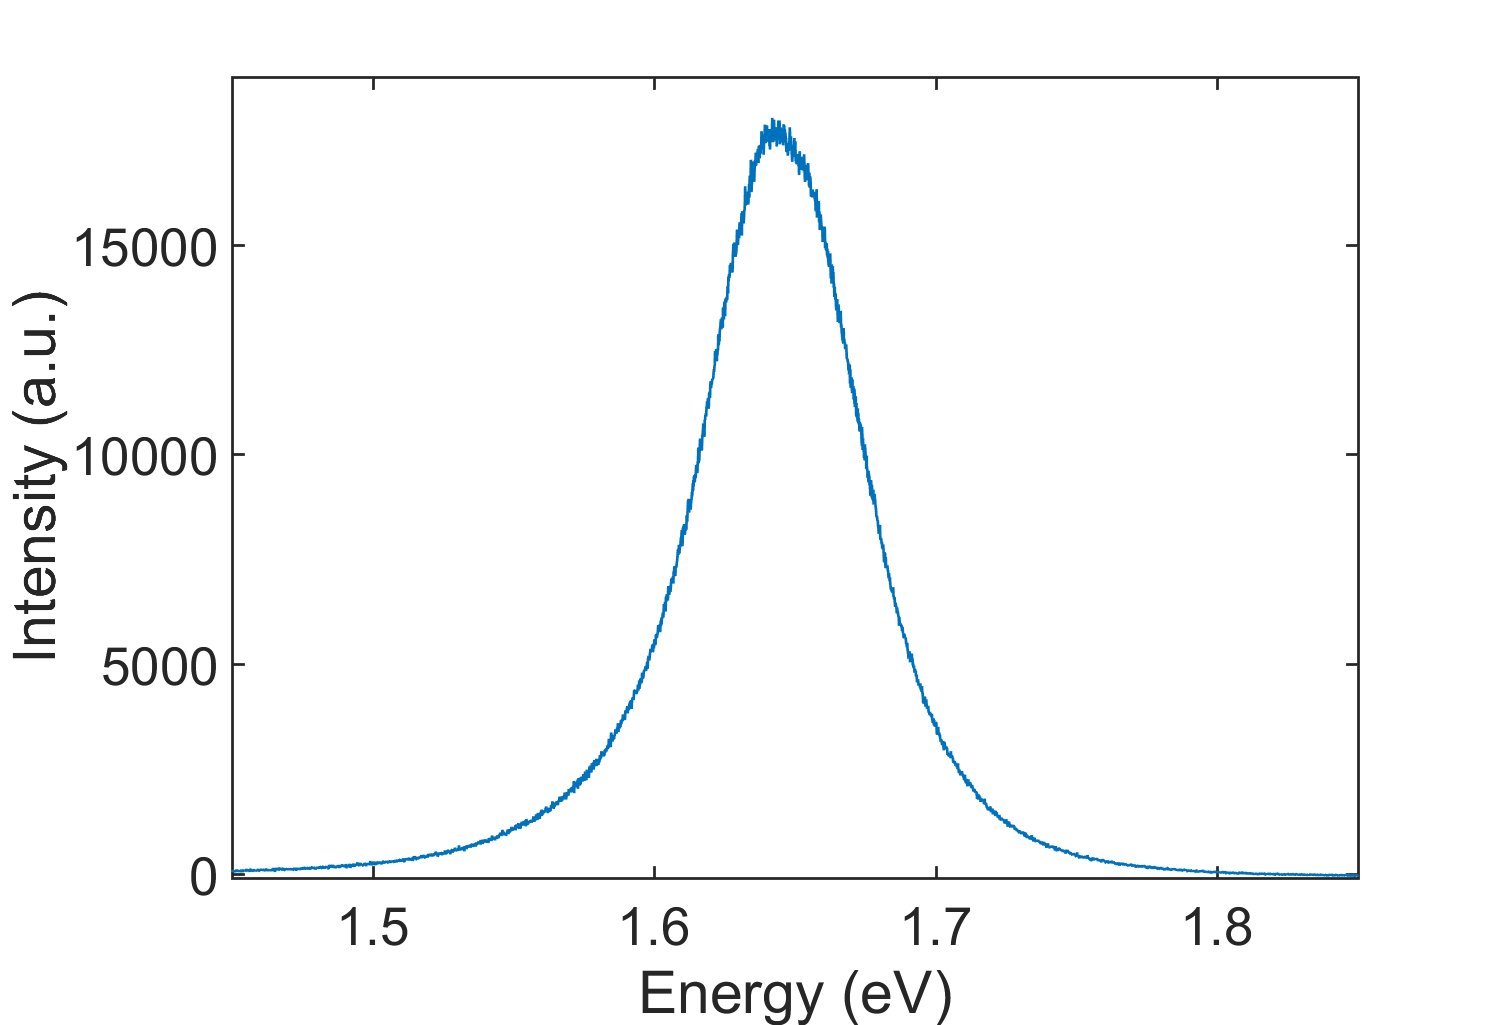
\includegraphics[scale=0.2]{WSe2/PLSpectrum.png}
			\caption{Typical PL spectrum from monolayer $WSe_2$}
			\label{fig:WSe2PLSpectrum}
		\end{subfigure}
		\qquad
		\begin{subfigure}[b]{0.4\textwidth}
			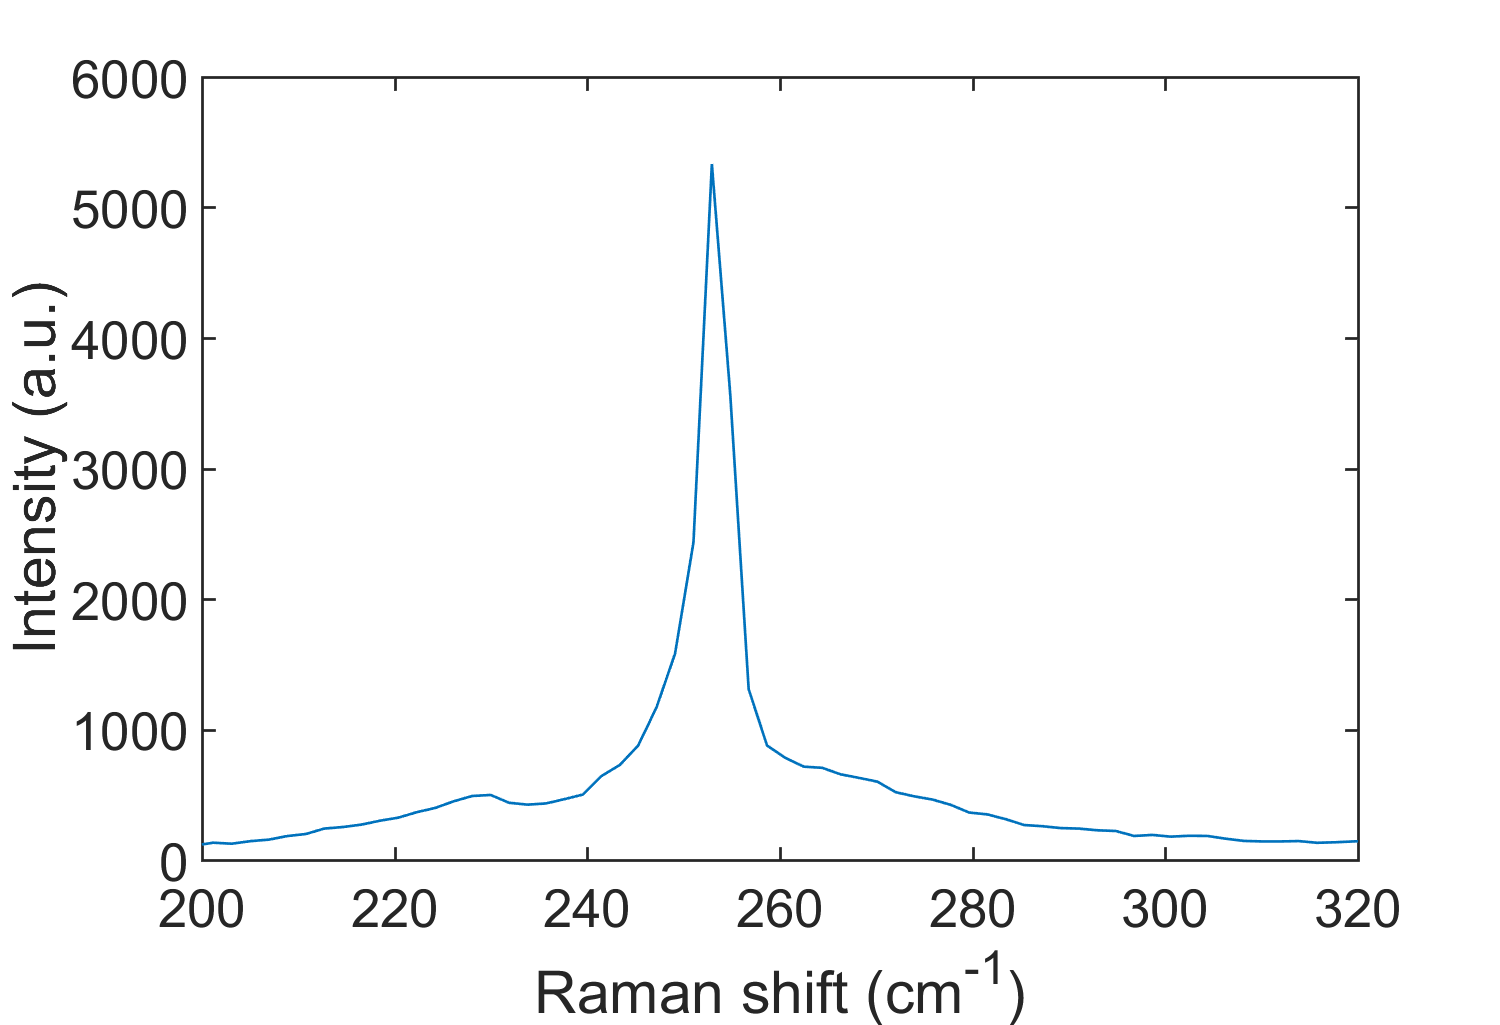
\includegraphics[scale=0.2]{WSe2/RamanSpectrum.png}
			\caption{Typical Raman spectrum from monolayer $WSe_2$}
			\label{fig:WSe2RamanSpectrum}
		\end{subfigure}
		\caption{PL and Raman spectra from monolayer $WSe_2$}
		\label{fig:WSe2PLRamanSpectra}
	\end{center}
\end{figure}
	
\begin{figure}[!h]
	\begin{center}
		\begin{subfigure}[b]{0.4\textwidth}
			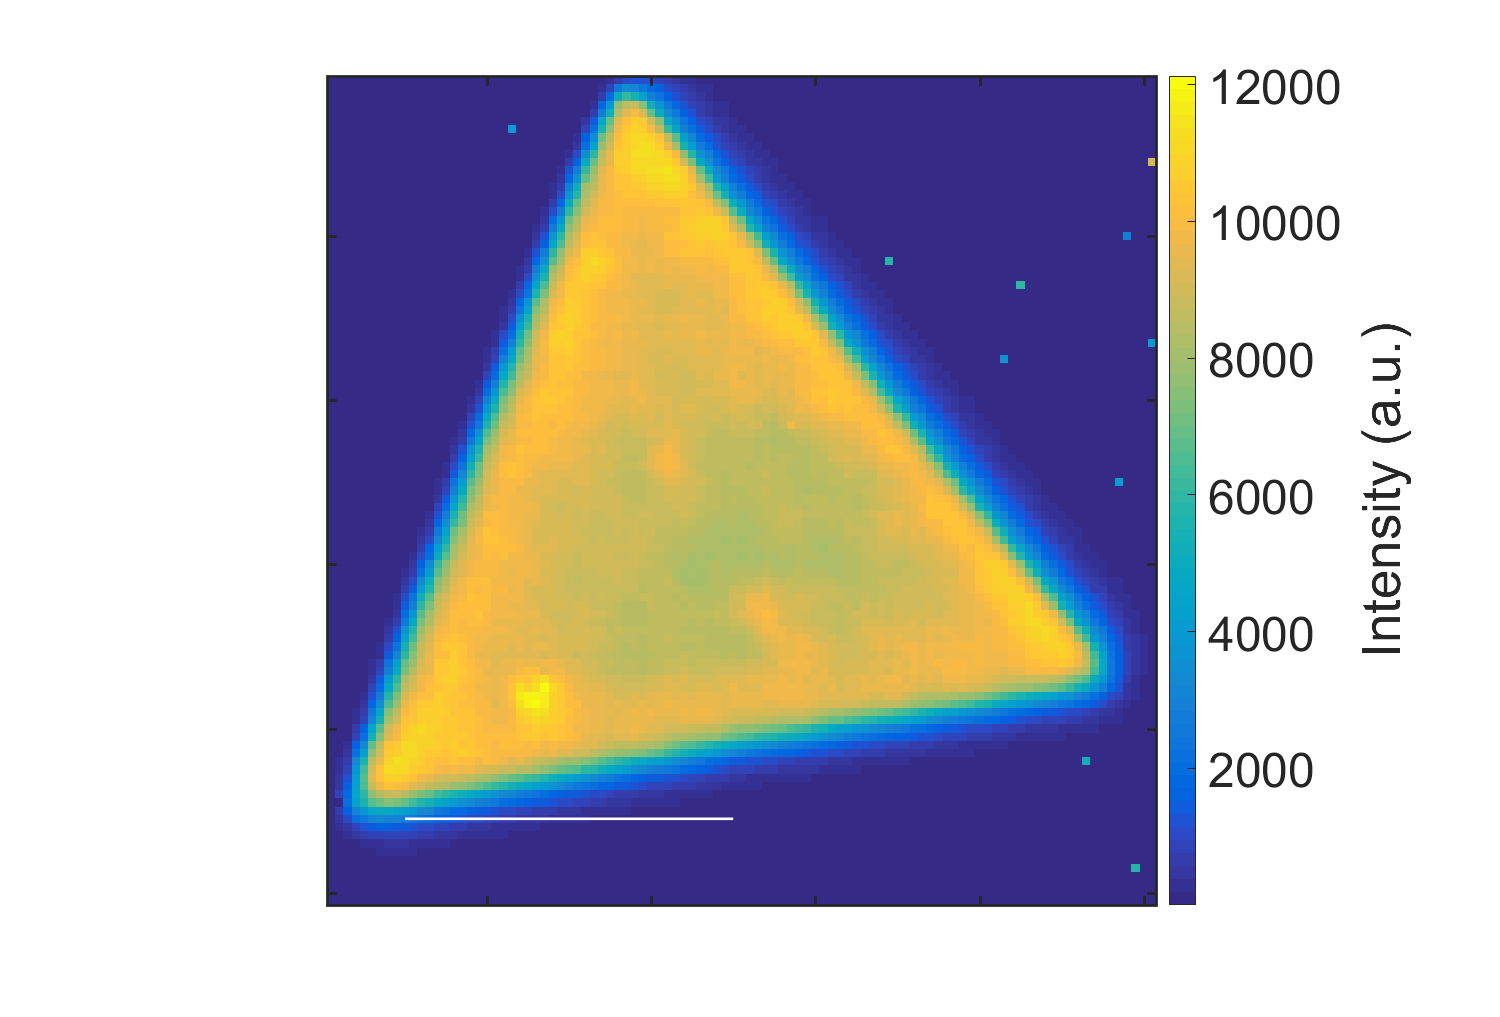
\includegraphics[scale=0.2]{WSe2/PLIntensity.png}
			\caption{PL intensity}
			\label{fig:WSe2PLIntensityMap}
		\end{subfigure}
		\qquad
		\begin{subfigure}[b]{0.4\textwidth}
			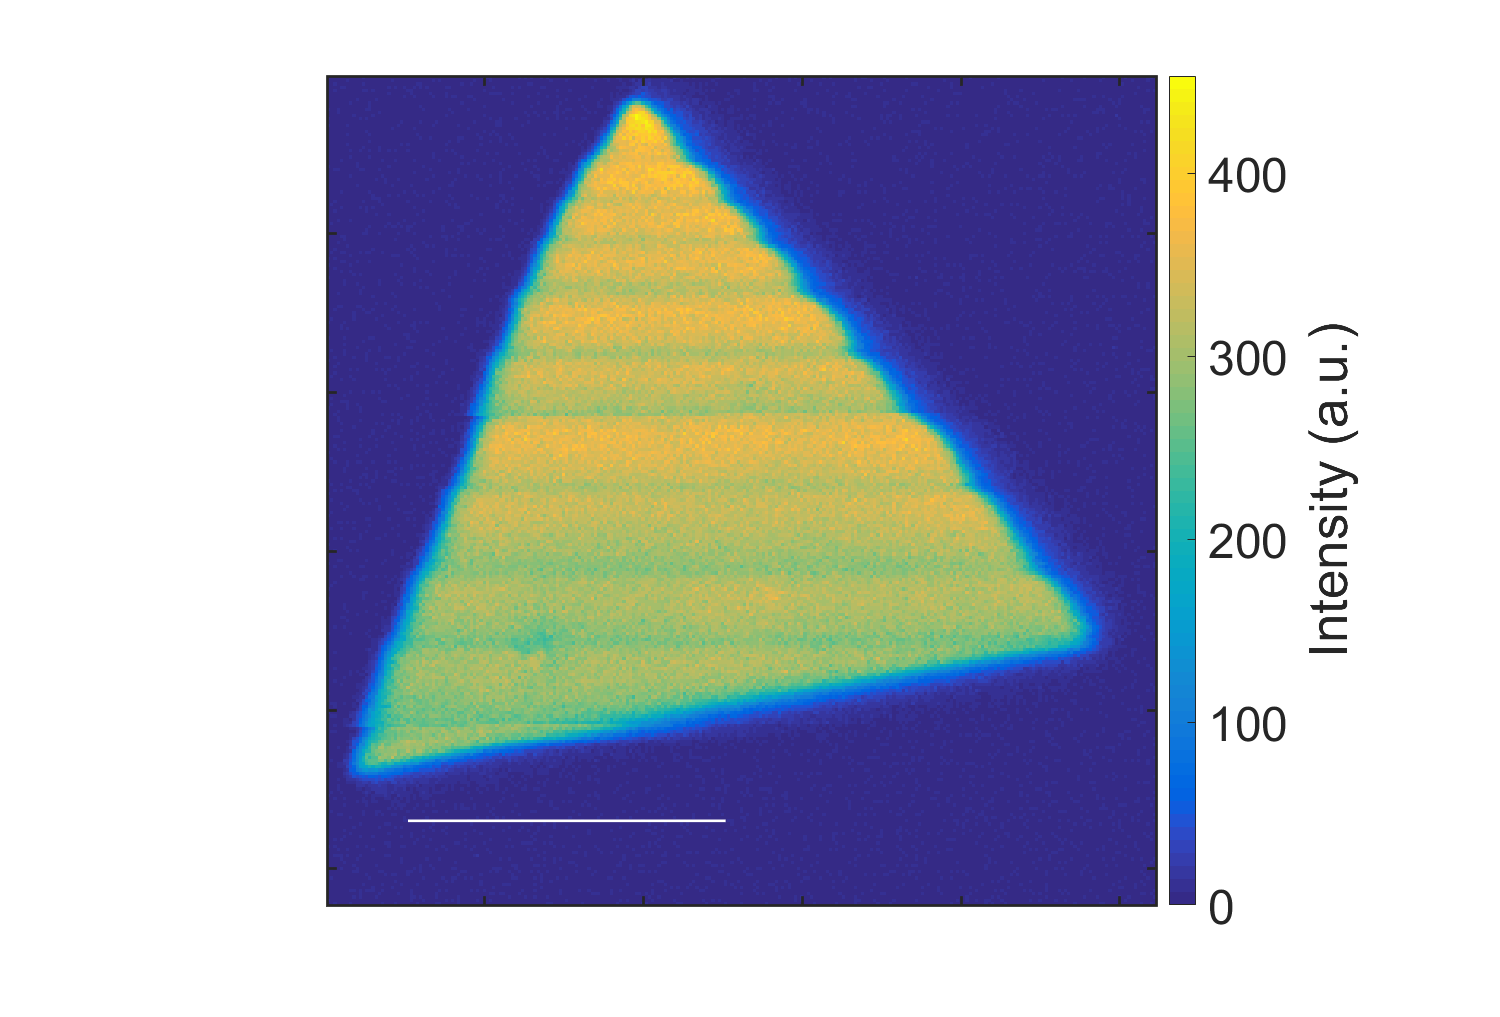
\includegraphics[scale=0.2]{WSe2/RamanEIntensity.png}
			\caption{Raman E intensity}
		\end{subfigure}
		\caption{PL intensity and Raman $E^1_{2g}$ intensity maps}
	\end{center}
\end{figure}

A typical map of PL intensity of a $WSe_2$ sample can be seen in Figure \ref{fig:WSe2PLIntensityMap}. The PL intensity is homogeneous throughout the flake. It does not exhibit the trisecting pattern as seen in $WS_2$ samples e.g. Figure \ref{fig:WSe2PLIntensityMap}.
	
\begin{figure}[!h]
	\begin{center}
		\begin{subfigure}[b]{0.3\textwidth}
			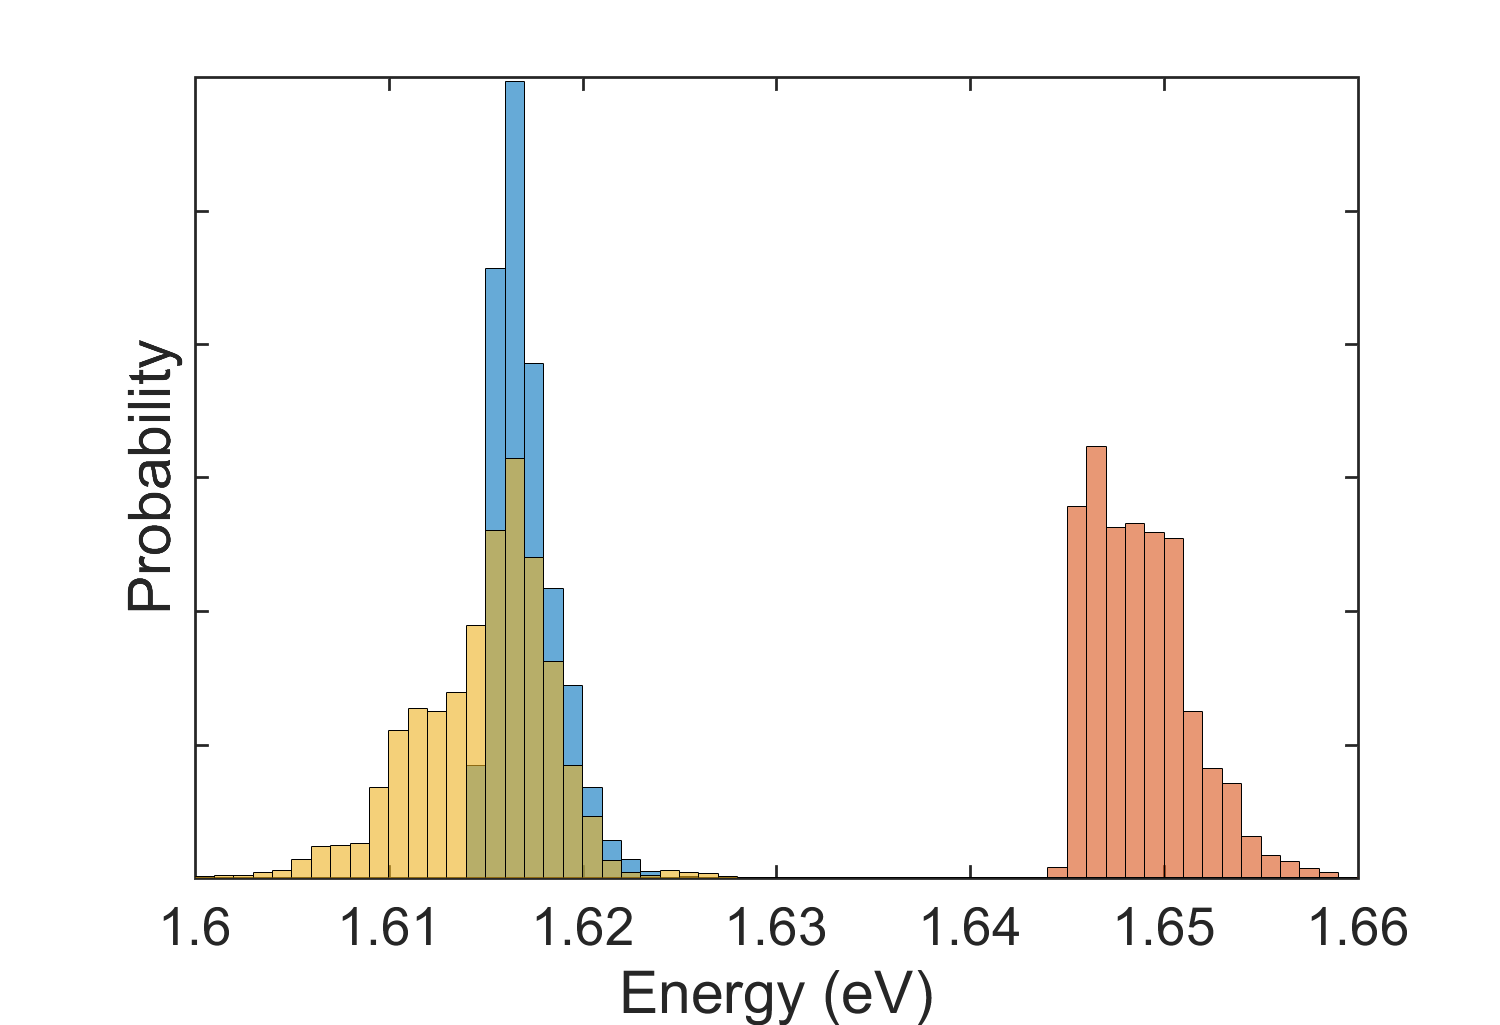
\includegraphics[scale=0.2]{WSe2/WSe2PositionHistograms.png}
			\caption{WSe2 PL peak positions histograms}
			\label{fig:WSe2PLPositionHistograms}
		\end{subfigure}
		\qquad
		\begin{subfigure}[b]{0.3\textwidth}
			\includegraphics[scale=0.2]{WSe2/Wse2WidthHistograms.png}
			\caption{WSe2 PL peak positions histograms}
			\label{fig:WSe2PLWidthHistograms}
		\end{subfigure}
		\caption{Comparison of PL peak positions and widths in different $WSe_2$ samples}
		\label{fig:WSe2PLHistograms}
	\end{center}
\end{figure}

A comparison of PL peak positions and widths between different samples of WSe2 can be seen in Figure \ref{fig:WSe2PLHistograms}.

\begin{figure}[!h]
	\begin{center}
		\begin{subfigure}[b]{0.4\textwidth}
			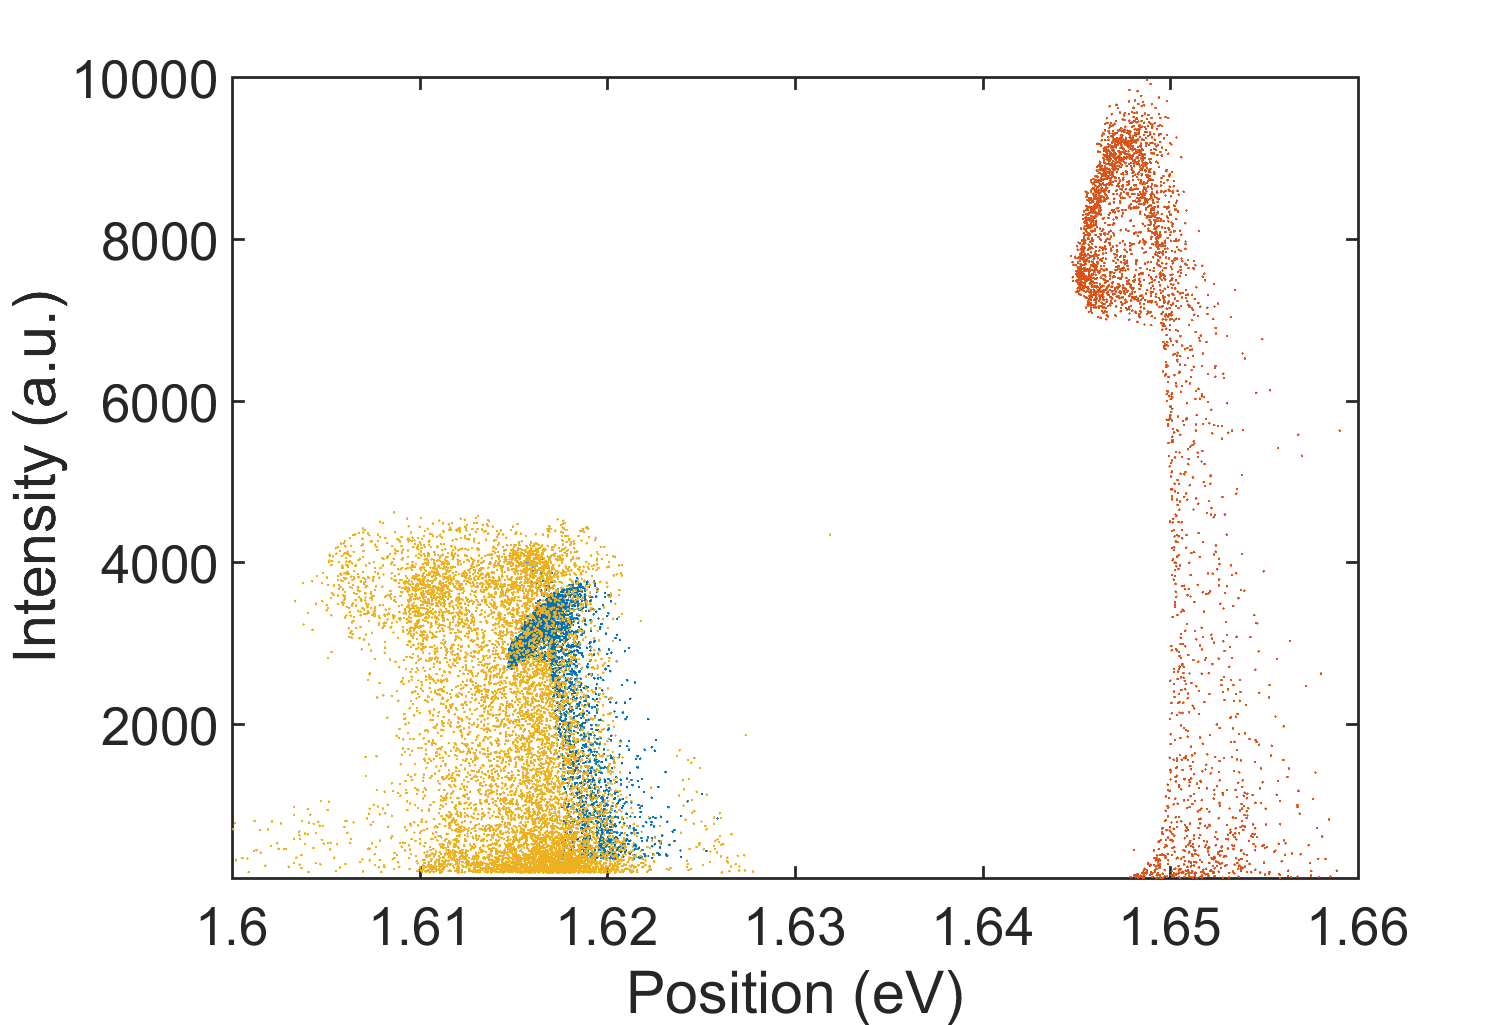
\includegraphics[scale=0.2]{WSe2/WSe2PositionIntensityScatterComparison.png}
			\caption{Intensity vs position}
			\label{fig:WSe2PositionIntensityScatterComparison}
		\end{subfigure}
		\qquad
		\begin{subfigure}[b]{0.4\textwidth}
			\includegraphics[scale=0.2]{WSe2/Wse2PositionWidthScatterComparison.png}
			\caption{Width vs position}
			\label{fig:WSe2PositionWidthScatterComparison}
		\end{subfigure}
		\caption{PL peak parameters distribution}
		\label{fig:WSe2ScatterComparison}
	\end{center}
\end{figure}

By plotting the intensity and width of the PL peaks against the peak position as seen in Figure \ref{fig:WSe2ScatterComparison} certain patterns can be observed. The intensity is generally mostly grouped around maximum values and relatively narrowly spread across the position spectrum. The thick flakes show much more even distribution of intensity across the position, which combined with the wide distribution of positions results in a much more inhomogeneous sample.  The width and positions are generally well grouped with flakes with smaller width having more narrow distribution than those with greater width. Also few-layer flake shows a smaller peak width. Overall there is no obvious relation between position and width. 

%% Raman

The Raman spectroscopy is a very useful characterisation technique for TMDCs. For most TMDCs it can be used to identify the number of layers or strain within the layer. However in the case of $WSe_2$ the position of the $E^1_{2g}$ and $A_{1g}$ largely overlaps and therefore it is difficult to accurately determine the difference in their position. Because of that this method of identifying the number of layers cannot be employed easily. It is however still possible to examine the strain within the layers by noting the shift of the $E^1_{2g}$ peak. A Raman $E^1_{2g}$ peak position distribution from a representative sample can be seen in Figure \ref{fig:WSe2RamanPositionHistogram1}. The strain can be then determined from the mean position of $250.678 \pm 0.095$ $cm^{-1}$  to be 2.44 {\%} \cite{Dadgar2018}.

\begin{figure}[!h]
	\begin{center}
		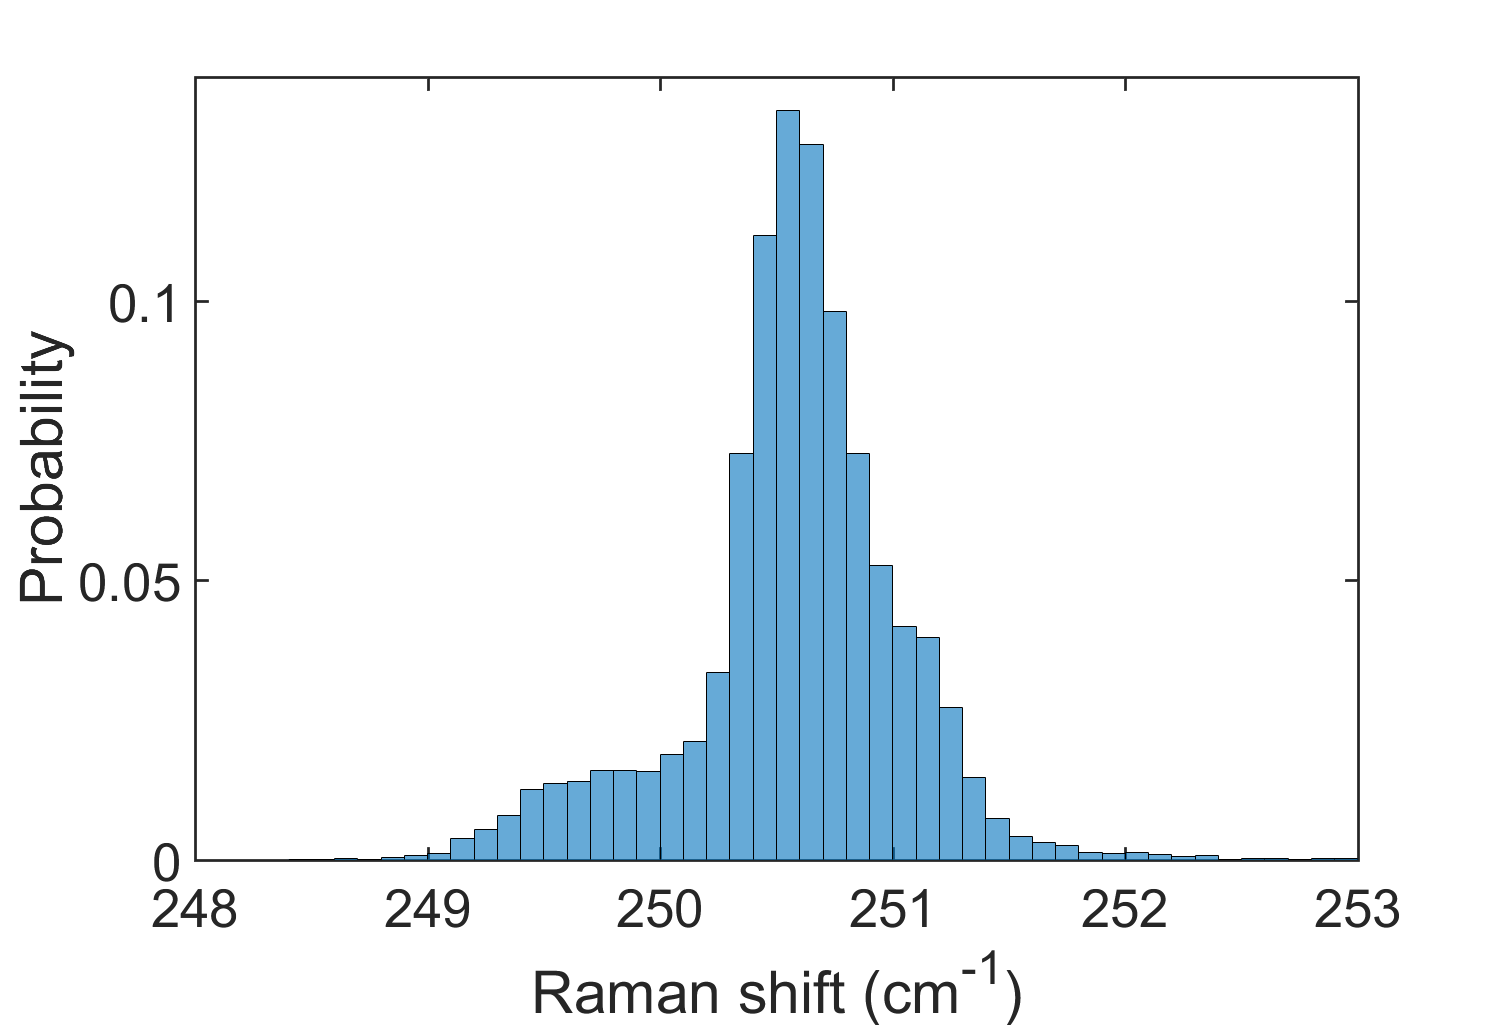
\includegraphics[scale=0.3]{WSe2/WSe2RamanPositionHistogram1.png}
		\caption{Histogram of Raman $E^1_{2g}$ peak position from monolayer $WSe_2$}
		\label{fig:WSe2RamanPositionHistogram1}
	\end{center}
\end{figure}


\begin{figure}[!h]
	\begin{center}
		\begin{subfigure}[b]{0.4\textwidth}
			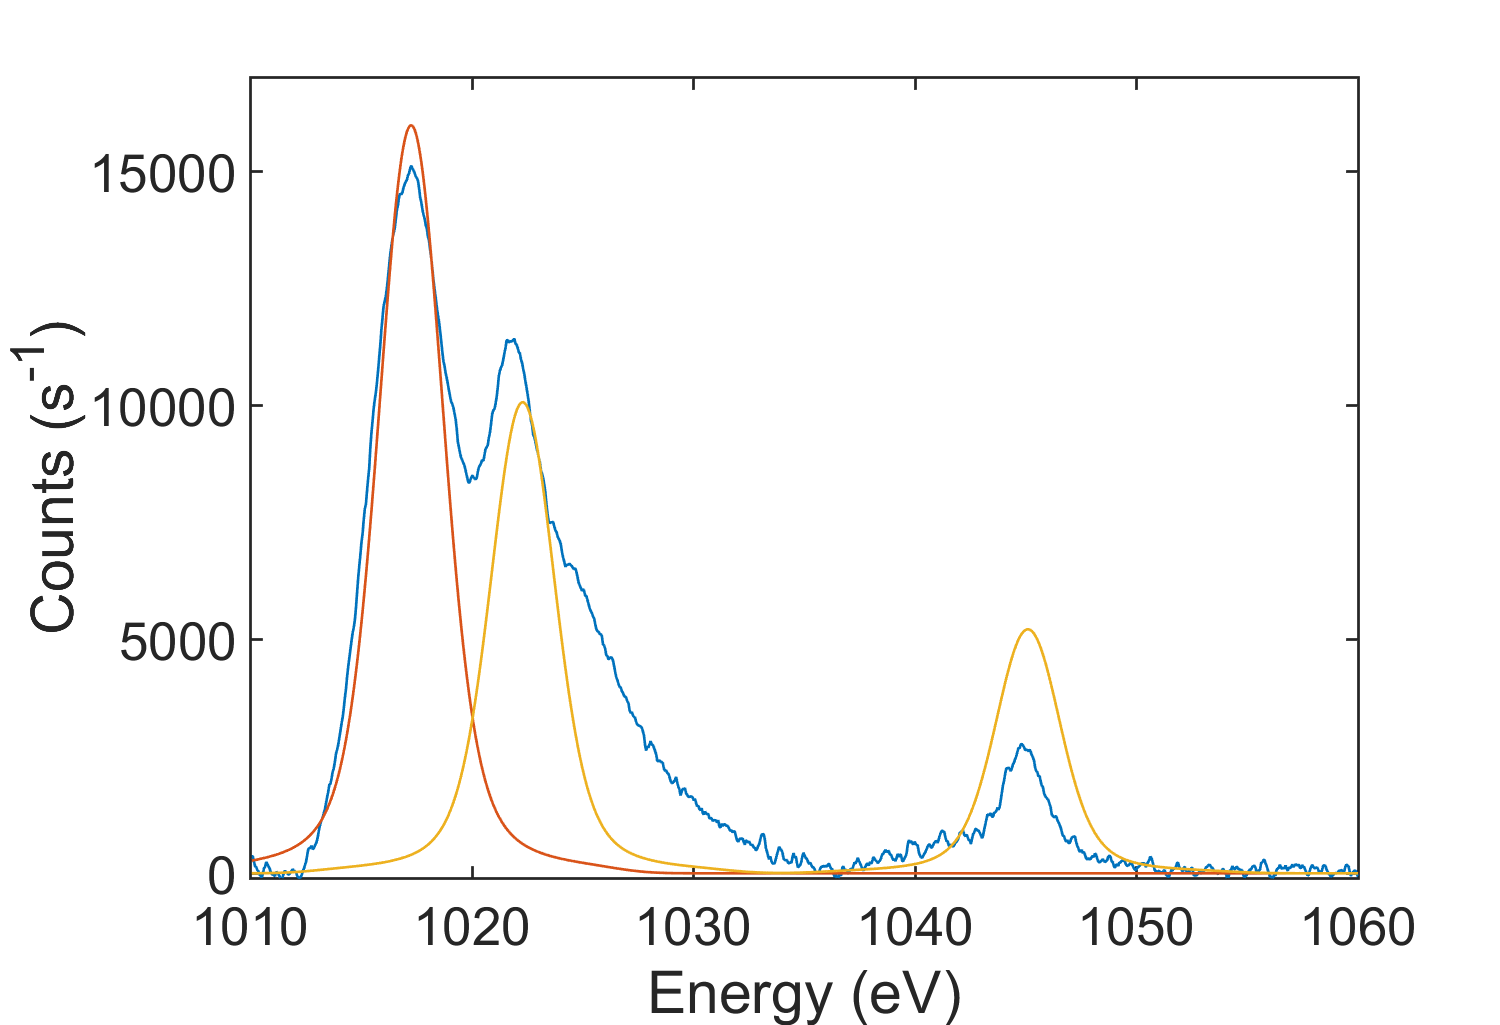
\includegraphics[scale=0.2]{WSe2/WSe2XPSThinZn.png}
			\caption{Thin flakes}
			\label{fig:WSe2XPSThinZn}
		\end{subfigure}
		\qquad
		\begin{subfigure}[b]{0.4\textwidth}
			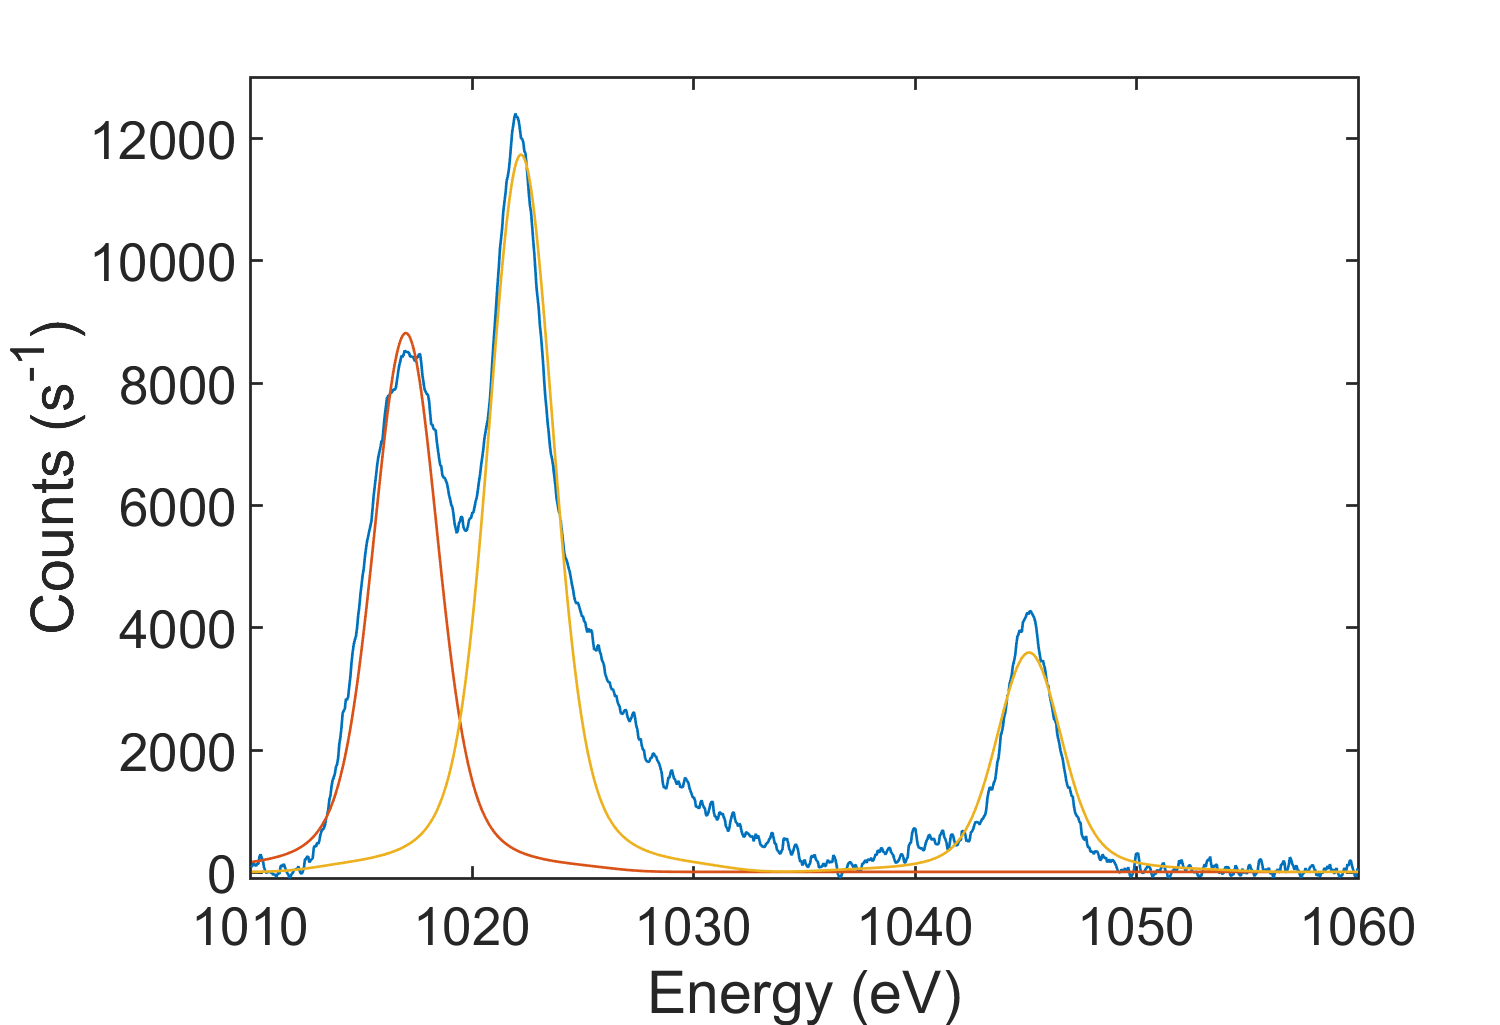
\includegraphics[scale=0.2]{WSe2/WSe2XPSThickZn.png}
			\caption{Thick flakes}
			\label{fig:WSe2XPSThickZn}
		\end{subfigure}
		
		\begin{subfigure}[b]{0.25\textwidth}
			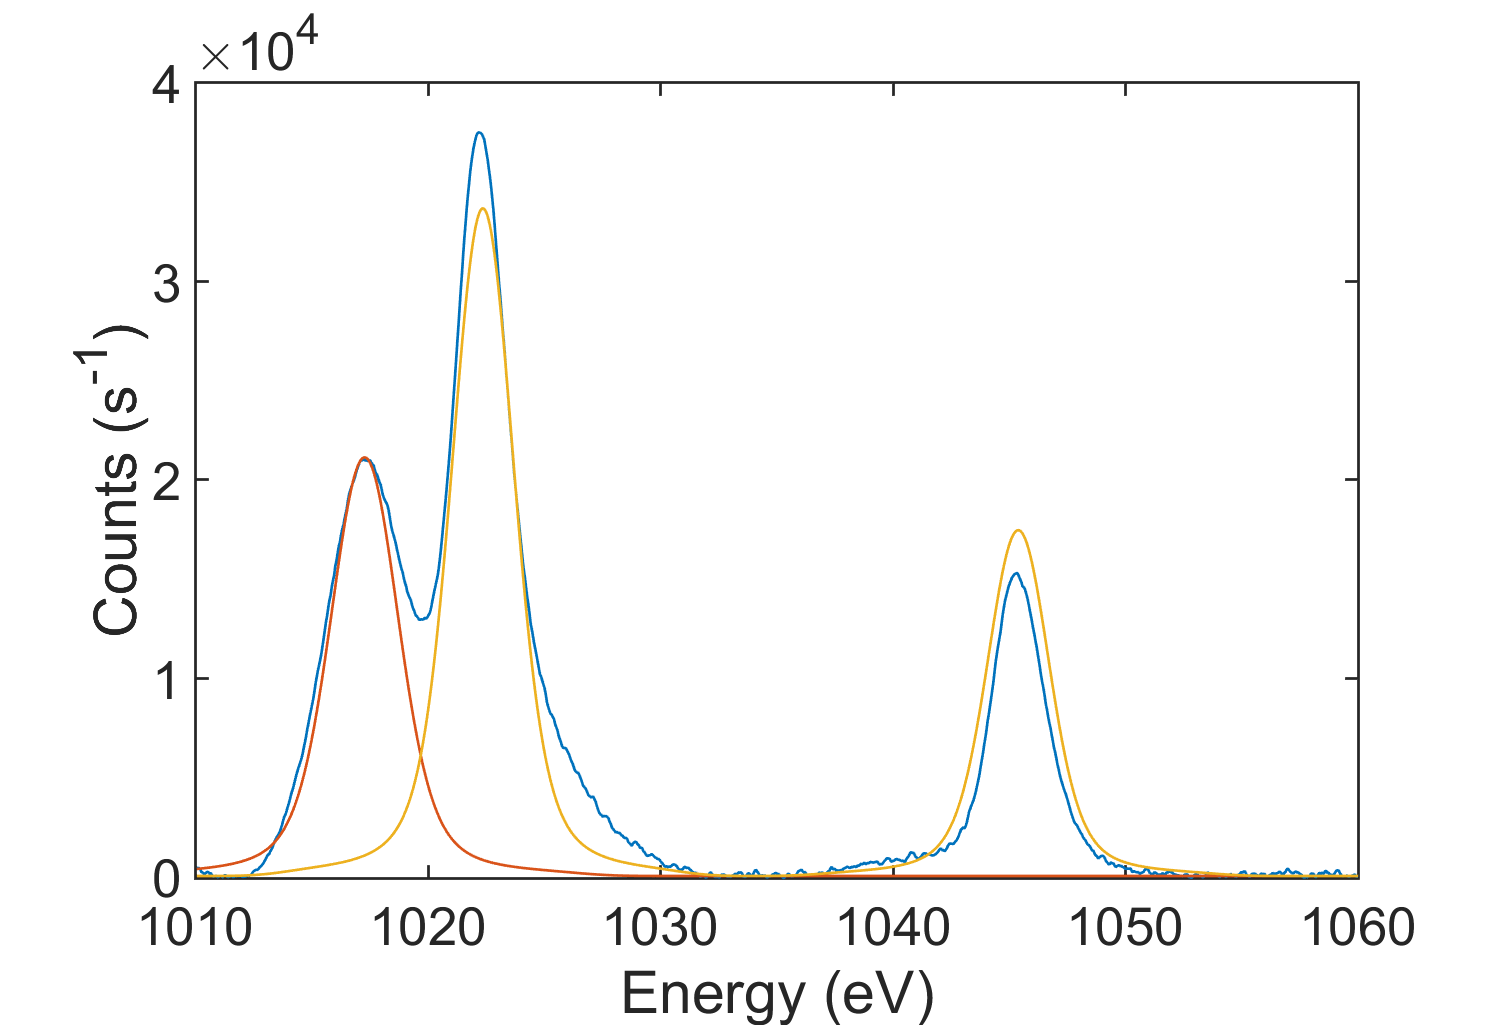
\includegraphics[scale=0.2]{WSe2/WSe2XPSRefZn.png}
			\caption{Empty area}
			\label{fig:WSe2XPSRefZn}
		\end{subfigure}
		\caption{XPS spectra around Zn2p peaks in different areas of the sample}
		\label{fig:WSe2XPSSpectra}
	\end{center}
\end{figure}

The samples has been characterised with XPS in order to test whether any Zn can be found in the sample and in what form. As seen in Figure \ref{fig:WSe2XPSSpectra} the Zn is present in all three areas investigated. The empty area with no flakes was measured as a reference (Figure \ref{fig:WSe2XPSRefZn}) and Zn has been found there. This indicates that there is some residue Zn covering the entire sample. 
